\begin{frame}
    \frametitle{Reactor Deployment}
    \begin{columns}
        \column[t]{5cm}
        \begin{itemize}
            \item The last \gls{LWR} is decommissied in 2076
            \item In the no growth scenarios (Scenarios 2 and 3) the advanced reactors are 
                  deployed starting in October 2031
            \item In the 1\% growth scenarios (Scenarios 4 and 5) the advanced reactors are 
                  deployed starting in March 2029
            \item The maximum number of advanced reactors deployed at one time 
                  in Scenarios 2-5 are 9182, 1225, 17656, and 2361 reactors, respectively
        \end{itemize}

        \column[t]{5cm}
        \vspace{-1cm}
        \begin{figure}
            \centering 
            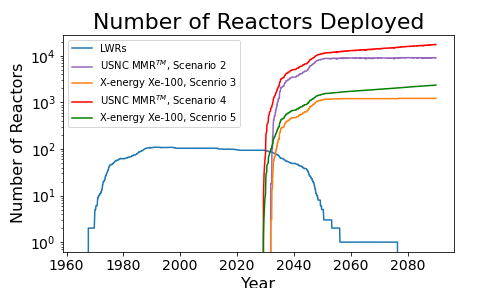
\includegraphics[scale=0.35]{figures/rxdeployment_scenarios_all.png}
            \caption{Reactor deployment schedule for \glspl{LWR} and 
            advanced reactors.}
            \label{fig:rx_deployment} 
        \end{figure}
    \end{columns}
\end{frame}

\begin{frame}
    \frametitle{Energy}
    \begin{columns}
        \column[t]{5cm}
        \begin{itemize}
            \item Energy produced by \glspl{LWR} in Scenario 1 in 2025 is 91.818 GWe-y
            \item Scenarios 2 and 3 do not meet demand between 2030-2050
            \item Scenarios 4 and 5 do not meet demand between 2026-2048
            \item Noticable deviations from demand in Scenarios 2, 4 when new 
                  reactors are deployed
            \item Initial gap between demand and energy produced is due to 
                  how the ManagerInst responds to the demand of the GrowthRegion
        \end{itemize}

        \column[t]{5cm}
        \vspace{-1.1cm}
        \begin{figure}
            \centering 
            \begin{subfigure}
                \centering
                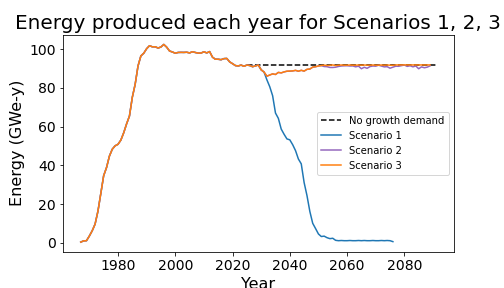
\includegraphics[scale=0.3]{figures/energy_scenarios_123.png}
                \label{fig:energy_123}
            \end{subfigure}
            \vspace{-0.7cm}
            \smallskip
            \begin{subfigure}
                \centering
                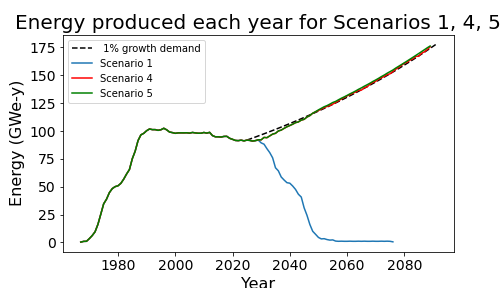
\includegraphics[scale=0.3]{figures/energy_scenarios_145.png}
                \label{fig:energy_145}
            \end{subfigure}
            \caption{Energy produced each year by all reactors in Scenarios 1-3 (top)
            and Scenarios 1, 4, 5 (bottom)}
            \label{fig:energy}
        \end{figure}
    \end{columns}
\end{frame}

\begin{frame}
    \frametitle{Uranium Mass Supply}
    \begin{columns}
        \column[t]{5cm}
            \begin{itemize}
                \item All scenarios have the same uranium demands until 
                      advanced reactors are deployed
                \item Large peaks in Scenarios 2 and 4 correspond to the 
                      deployment of new reactors
                \item Less variation with time in the uranium supplied to reactors
                      for Scenarios 3 and 5 than Scenarios 2 and 4
            \end{itemize}
        \column[t]{5cm}
        \vspace{-0.8cm}
        \begin{figure}
            \centering 
            \begin{subfigure}
                \centering
                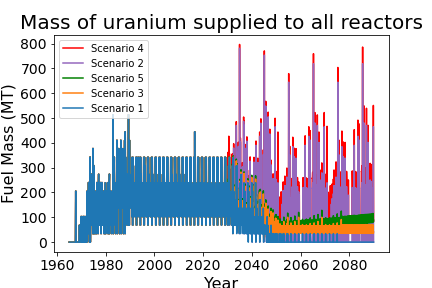
\includegraphics[scale=0.3]{figures/fuelsupply_scenarios_all.png}
                \label{fig:fuel_all}
            \end{subfigure}
            \begin{subfigure}
                \centering
                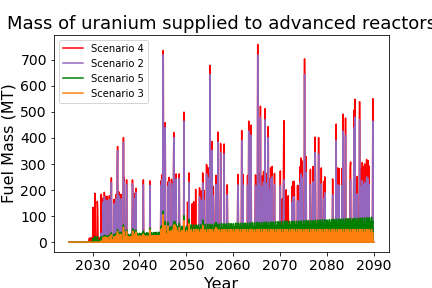
\includegraphics[scale=0.3]{figures/advancedRX_fuelsupply_scenarios_2-5.png}
                \label{fig:fuel_advancedRX}
            \end{subfigure}
            \caption{Uranium mass sent to all reactors (top)
            and only advanced reactors (bottom)}
            \label{fig:fuel}
        \end{figure}
    \end{columns}
    

\end{frame}

\begin{frame}
    \frametitle{\gls{SWU} Requirements}
    \begin{columns}
        \column[t]{5cm}
            \begin{itemize}
                \item Follows similar pattern to uranium mass 
                \item Scenarios 2 and 4 require the most \gls{SWU} 
                      because of the large mass of urnaium, despite a 
                      lower enrichment level for the advanced reactors 
                      Scenarios 3 and 5
                
            \end{itemize}
        \column[t]{5cm}
        \vspace{-1cm}
        \begin{figure}
            \centering 
            \begin{subfigure}
                \centering
                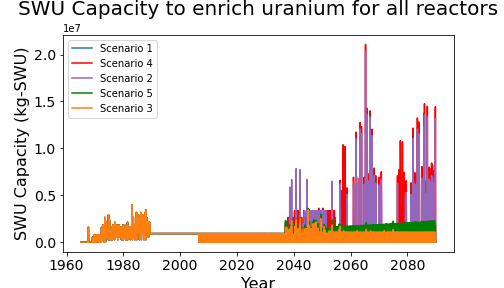
\includegraphics[height=0.35\textheight]{figures/totalswu_scenarios_all.png}
                \label{fig:swu_all}
            \end{subfigure}
            \vspace{-0.5cm}
            \begin{subfigure}
                \centering
                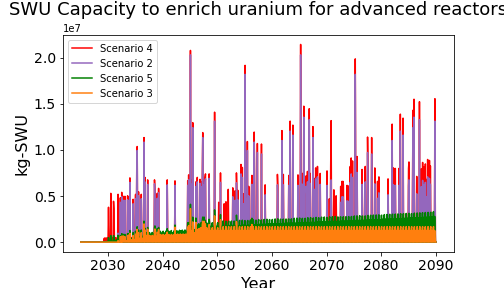
\includegraphics[height=0.35\textheight]{figures/haleuSWU_scenarios_all.png}
                \label{fig:swu_haleu}
            \end{subfigure}
            \caption{\gls{SWU} required to produce enriched uranium for all 
            reactors (top) and only advanced reactors (bottom)}
            \label{fig:swu}
        \end{figure}
    \end{columns}
    

\end{frame}

